
\begin{frame}{Content}{}
\tableofcontents
\end{frame}

%-------------------------------------------------------
%-------------------------------------------------------
\section{Introduction}
%-------------------------------------------------------
%-------------------------------------------------------

\begin{frame}
  \frametitle{Hadron vs. Lepton colliders}
  
  \begin{block}{}
    \centering
    Discovery to Precision
  \end{block}

  \begin{columns}
    \column{0.5\textwidth}
    \centering
    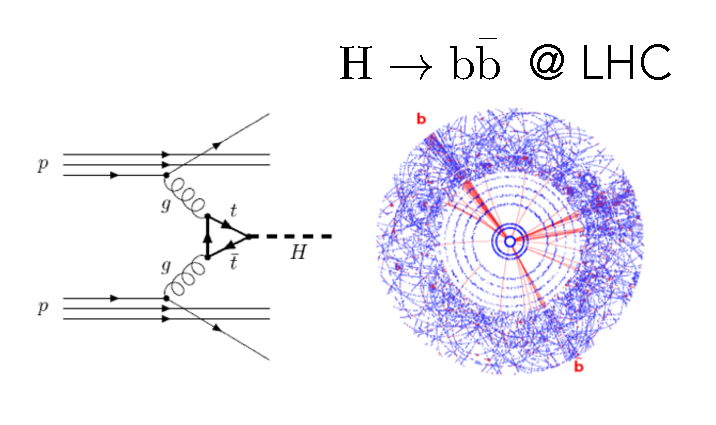
\includegraphics[width=\textwidth]{figures/hadronColliders.pdf}

    \begin{itemize}
    \item Protons are 
    \end{itemize}

    \column{0.5\textwidth}
    \centering
    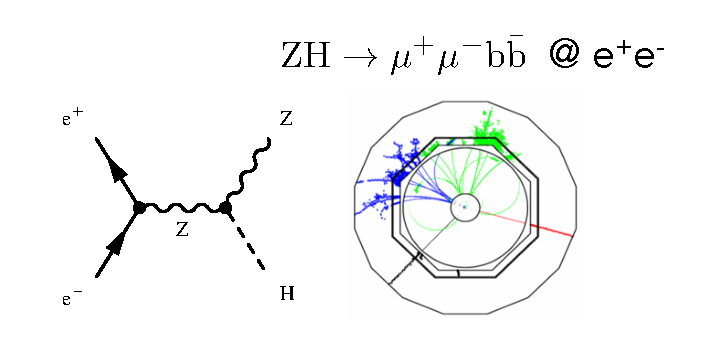
\includegraphics[width=\textwidth]{figures/leptonColliders.pdf}

  \end{columns}

\end{frame}

%-------------------------------------------------------
\subsection{CLIC}
%-------------------------------------------------------
\begin{frame}
  \frametitle{The Compact LInear Collider (CLIC)}

 
  \begin{itemize}
  \item A concept for an $e^{+}e^{-}$ linear collider for the post
    HL-LHC period.
  \item Energy range $\sqrt{s}$ : \textcolor{blue}{$380\,\gev$} to
    \textcolor{blue}{$3\,\tev$}
    \begin{itemize} 
    \item Two-beam acceleration scheme with gradients of $\sim$100~MV/m.
    \end{itemize}
  \end{itemize}
  
  \begin{columns} 
    \column{0.5\textwidth}
    
    \begin{itemize}
    \item Precision measurements of:
      \begin{itemize}
      \item Standard Model processes (Higgs, top).
      \item New physics potentially discovered at 13~TeV LHC.
      \item Search for new physics: unique sensitivity to particles with
        electroweak charge.
      \end{itemize}
    \end{itemize}

    \column{0.5\textwidth} \centering
    \begin{tikzpicture}
      \node[anchor=south west,inner sep=0] (image) at (0,
      0){\includegraphics[width=\textwidth]{../figures/CLIC/staging.pdf}};
      \begin{scope}[x={(image.south east)},y={(image.north west)}]
        \node[above, color=white] at (0.5, 0.001) {\textbf{48 km tunnel at 3 TeV stage}};
      \end{scope}
    \end{tikzpicture}
  \end{columns}

\end{frame}

%-------------------------------------------------------
\subsection{CLIC beam profile}
\begin{frame}
  \frametitle{Beam profile for CLIC}

 \begin{columns}
    \column{0.5\textwidth}
    \begin{tikzpicture}
      \node[anchor=south west,inner sep=0] (image) at (0,
      0){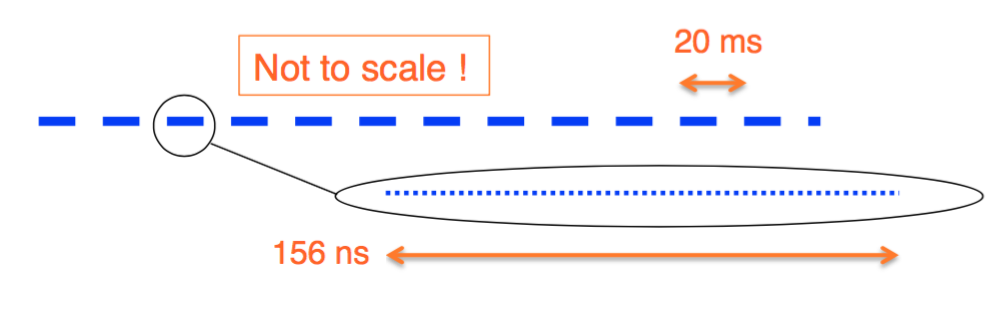
\includegraphics[width=\textwidth]{figures/CLICbeam.png}};
      \begin{scope}[x={(image.south east)},y={(image.north west)}]
        \node[above, color=blue] at (0.5, 0.9) {\textbf{CLIC bunch
            structure}};
        % \node[above, color=Orange] at (0.65, 0.05) {\tiny{1 train=312 bunches
        %     with 0.5~ns spacing}};
      \end{scope}
    \end{tikzpicture}

    \begin{itemize}
    \item 1 train consists of \textcolor{blue}{312} bunches with \textcolor{blue}{0.5}~ns spacing.
    \end{itemize}

    \centering
    \resizebox{0.9\columnwidth}{!}{\begin{tabular}{l c c} 
                                     \toprule 
                                     & CLIC at $\sqrt{s}=3\,\tev$ & LHC at $\sqrt{s}=13\,\tev$\\
                                     \midrule
                                     Colliding particles & electron-positron & proton-proton \\
                                     Instantaneous luminosity $\mathcal{L}$ & $6\times10^{34}$ \inversecmsquaredsec & $1\times10^{34}$ \inversecmsquaredsec \\
                                     Bunch-crossing separation & 0.5~ns & 25~ns \\
                                     Bunches per train & 312 & Not applicable \\
                                     Train duration & 156~ns & Not applicable \\
                                     Train repetition & 50~Hz & Not applicable \\
                                     IP size in x / y / z directions & 45~nm / 1~nm / $44\,\micron$ & $15\,\micron$ / $15\,\micron$ / 50~cm \\
                                     \bottomrule
                                   \end{tabular}}

    \column{0.5\textwidth}
    \centering
    \begin{itemize}
    \item \textcolor{red}{Bunch separation and train duration: drive timing resolution requirements for the detectors.}
    \item \textcolor{green}{Very small beam sizes at the interaction
        point} $\Rightarrow$ beam-induced backgrounds:
      \begin{itemize}
      \item \textcolor{blue}{$e^{+}e^{-}$ pairs}: low \pT, forward peaked, limits the inner radius of the VXD.
      \item \textcolor{blue}{$\gamma\gamma\rightarrow$hadrons}: larger \pT particles.
      \end{itemize}      
    \end{itemize}

  \end{columns}

  \begin{itemize}
  \item Short train duration implies:
    \begin{itemize}
    \item triggerless readout of the detectors.
    \item power pulsing: allows to reduce the average power dissipation.
    \end{itemize}
  \end{itemize}

\end{frame}

%-------------------------------------------------------
%-------------------------------------------------------
\section{Requirements}
\begin{frame}
  \frametitle{Requirements for the vertex detector}
\end{frame}


%-------------------------------------------------------
%-------------------------------------------------------
\section{R\&D on sensor and readout technologies}
%-------------------------------------------------------
\subsection{Thin planar sensors}
\begin{frame}
  \frametitle{Thin planar sensors}
\end{frame}
%-------------------------------------------------------
\subsection{The Timepix3 hybrid readout ASIC}
\begin{frame}
  \frametitle{The Timepix3 hybrid readout ASICs}
\end{frame}
%-------------------------------------------------------
\begin{frame}
  \frametitle{Assembly calibration}
\end{frame}

%-------------------------------------------------------
%-------------------------------------------------------
\section{Simulation}
\begin{frame}
  \frametitle{Simulation and reconstruction}
\end{frame}


%-------------------------------------------------------
%-------------------------------------------------------
\section{Timepix3 beam telescope}
\begin{frame}
  \frametitle{Timepix3 beam telescope}
\end{frame}

%-------------------------------------------------------
%-------------------------------------------------------
\section{Thin sensors studies}
\begin{frame}
  \frametitle{Thin sensors studies}
\end{frame}

%-------------------------------------------------------
%-------------------------------------------------------
\section{Active edge sensors}
\begin{frame}
  \frametitle{Active edge sensors}
\end{frame}

%-------------------------------------------------------
%-------------------------------------------------------
\label{lastslide}
\section{Conclusions}
\begin{frame}
  \frametitle{Conclusions}
\end{frame}